\documentclass[oneside,envcountsame,envcountchap,openany]{svmono}
\usepackage[utf8]{inputenc}
\usepackage{tikz}			% para gráficos e desenhos
\usetikzlibrary{calc}		% para cálculos em gráficos
\usepackage{fancyhdr}
\usepackage{makeidx}         % permite geracao de indice
% Definição de comandos personalizados
% Definição de ordinal masculino e feminino
\usepackage{etoolbox} % para garantir compatibilidade em várias situações
\usepackage{pdfpages}		 % para incluir pdfs
\usepackage{tocloft} 		 % para formatar o sumário
% Pacotes de hiperlinks
\usepackage{hyperref}
\hypersetup{
	colorlinks,
	citecolor=blue,
	filecolor=magenta,
	linkcolor=blue,
	urlcolor=cyan
}

\DeclareRobustCommand{\subsup}[1]{%
  \textsuperscript{%
    \tikz[baseline=(char.base)]{
      \node[inner sep=0.5pt, anchor=base] (char) {\textnormal{#1}};
      \draw[line width=0.3pt, yshift=-0.2ex]
        ($(char.south west)!0.15!(char.south east)$) --
        ($(char.south west)!0.85!(char.south east)$);
    }%
  }%
}
\DeclareRobustCommand{\ordm}[1]{#1\subsup{o}} % ordinal masculino
% Pacotes de formatação e layout
\usepackage[top=1in,left=2.5cm,bottom=1in,right=2.5cm]{geometry}
\title{Documentos Oficiais}
\begin{document}
\pagestyle{empty}
\thispagestyle{empty}

A seguinte documentação oficial relativa ao processo de reforma curricular encontra-se apensada nas
páginas a seguir:

\begin{enumerate}
      \item \textbf{Câmara de Educação Superior do Conselho Nacional de Educação}  \\
            \textbf{RESOLUÇÃO CNE/CES \ordm{n}~5, DE 16 DE NOVEMBRO DE 2016} \\
            Institui as Diretrizes Curriculares Nacionais para os cursos de graduação na área da Computação, abrangendo os cursos de bacharelado em Ciência da Computação, em Sistemas de Informação, em \textbf{Engenharia de Computação}, em Engenharia de Software e de licenciatura em Computação, e dá outras providências (pág.~\pageref{cne2016}).

      \item \textbf{Sociedade Brasileira de Computação (SBC)}  \\
            \textbf{Referenciais de Formação para os Cursos de Graduação em Computação –-- 2017} \\
            Documento elaborado com base na Resolução CNE/CES \ordm{n}~5/2016, com o objetivo de orientar a estrutura curricular dos cursos da área de Computação, considerando competências, conteúdos e práticas pedagógicas atualizadas (pág. \pageref{sbc2017}).

      \item \textbf{Câmara de Educação Superior do Conselho Nacional de Educação} \\
            \textbf{RESOLUÇÃO \ordm{n}~7, DE 18 DE DEZEMBRO DE 2018} \\
            Estabelece as Diretrizes para a Extensão na Educação Superior Brasileira e regimenta o disposto na Meta 12.7 da Lei \ordm{n}~13.005/2014, que aprova o Plano Nacional de Educação –-- PNE –-- 2014-2024 e dá outras providências (pág. \pageref{rcne2018}).

      \item \textbf{Universidade do Estado do Rio de Janeiro}  \\
            \textbf{Deliberação \ordm{n}~33, DE 28 DE DEZEMBRO DE 1995} \\
            Dispõe sobre as Normas Gerais de Ensino de Graduação da UERJ (pág. \pageref{delib3395}).

      \item \textbf{Universidade do Estado do Rio de Janeiro}  \\
            \textbf{Deliberação \ordm{n}~59, DE 12 DE DEZEMBRO DE 2019} \\
            Altera o Capítulo II, artigos 56, 57 e seu parágrafo único, da Deliberação \ordm{n}~33/1995, que trata das normas gerais de Ensino de Graduação da UERJ (pág. \pageref{delib592019}).
      \item \textbf{Universidade do Estado do Rio de Janeiro}  \\
            \textbf{Deliberação \ordm{n}~04, DE 13 DE ABRIL DE 2023}  \\
            Dispõe sobre a inserção curricular da extensão nos cursos da UERJ e dá outras providências (pág. \pageref{del4}).
      \item \textbf{CONFEA – Conselho Federal de Engenharia e Agronomia} \\
            \textbf{RESOLUÇÃO \ordm{n}~380, DE 17 DE DEZEMBRO DE 1993}  \\
            Discrimina as atribuições provisórias dos Engenheiros de Computação ou Engenheiros Eletricistas com ênfase em Computação e dá outras providências. Brasília: Diário Oficial da União, Seção I, página 193, 06 de janeiro de 1994 (pág. \pageref{confea1993}).
\end{enumerate}
\pagestyle{empty}
\thispagestyle{empty}
% Legislação
% Institui as Diretrizes Curriculares Nacionais para os cursos de graduação na área da Computação
\chapter{Resolução CNE/CES n\textordmasculine{} 5, de 16 de novembro de 2016}
\label{cne2016}
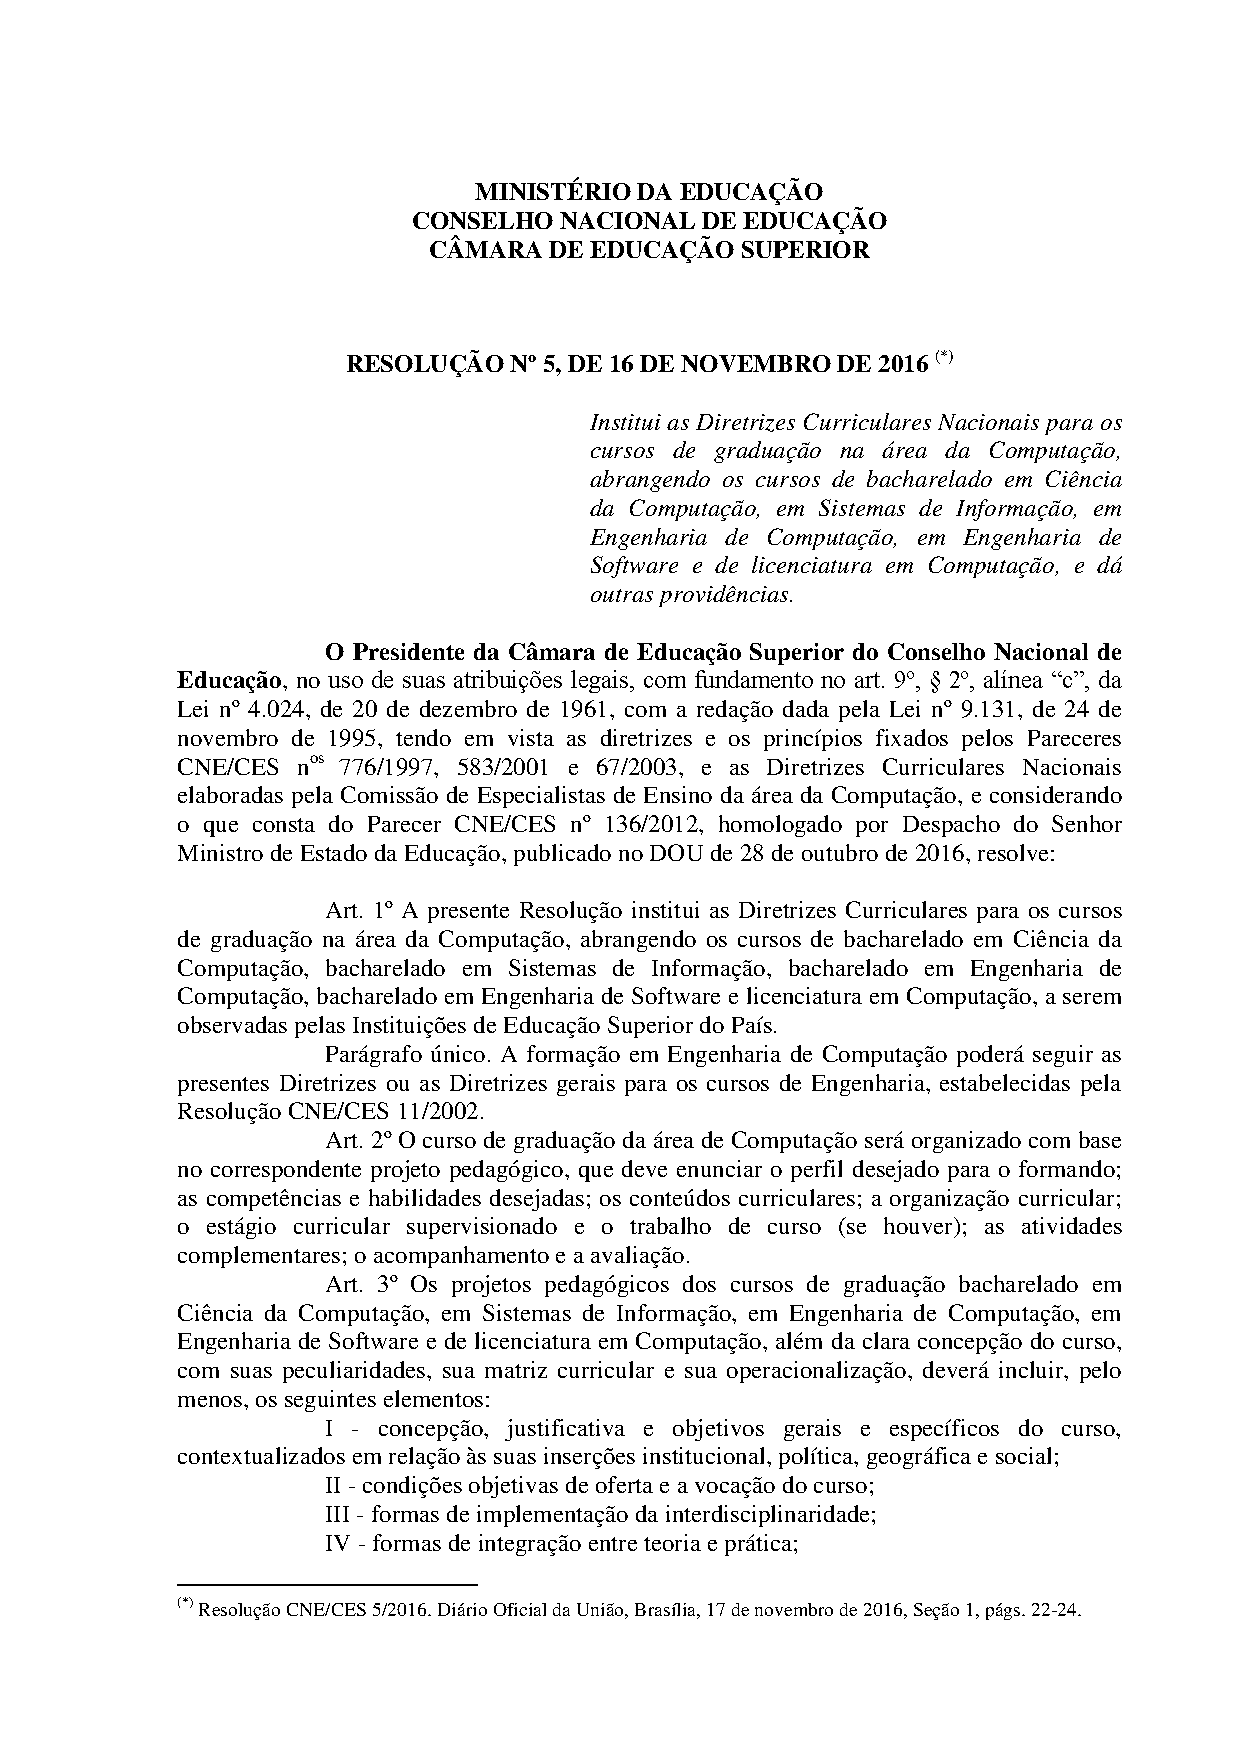
\includepdf[pages=-,pagecommand={\thispagestyle{empty}}]{leis/rces005_16.pdf}
% Referenciais SBC para cursos de Computação
\chapter{SBC: Referenciais para Graduação em Computação}
\label{sbc2017}
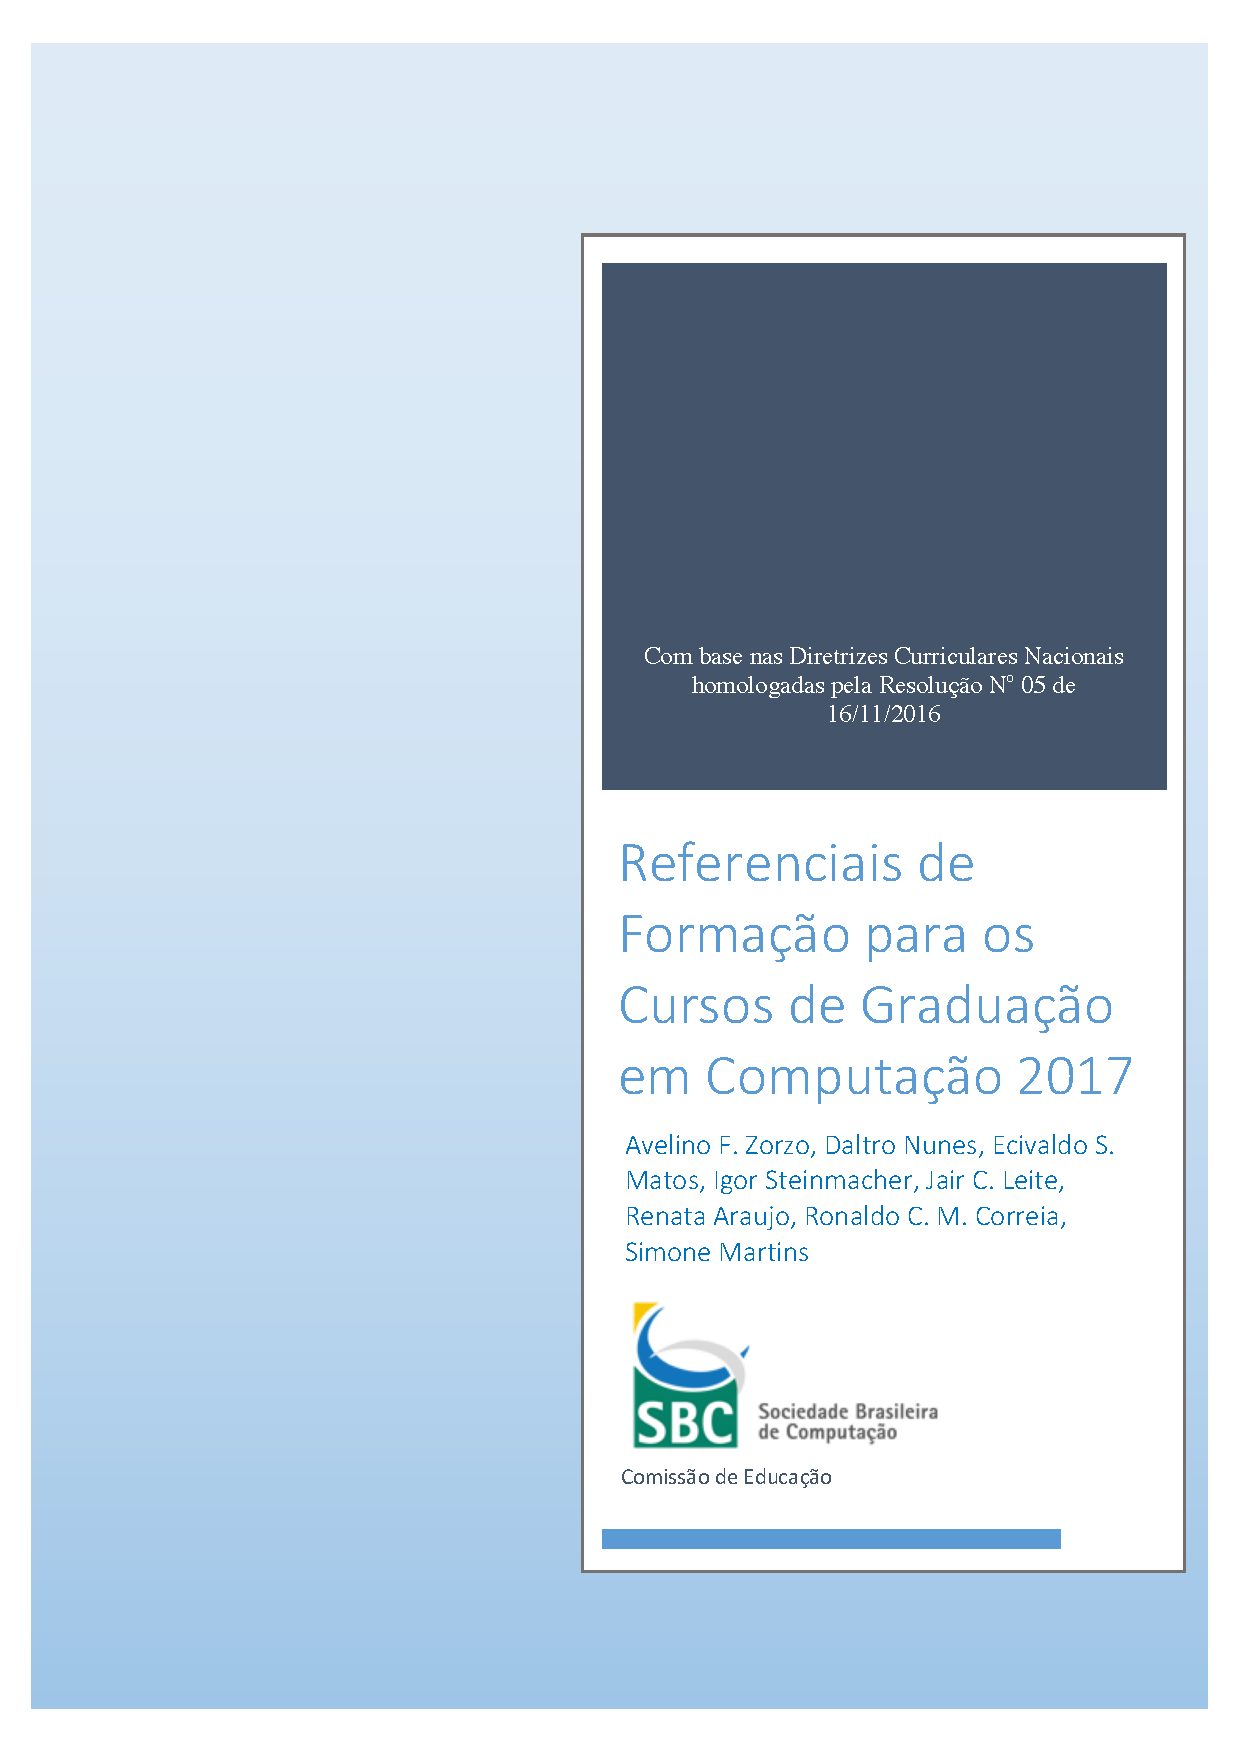
\includepdf[pages=-,pagecommand={\thispagestyle{empty}}]{leis/sbc2017.pdf}
% Resolução CNE/CES n. 7/2018, que estabelece as as Diretrizes para a Extensão na Educação Superior Brasileira
\chapter{Resolução n\textordmasculine{} 7, de 18 de dezembro de 2018 - CNE/CES}
\label{rcne2018}
\includepdf[pages=-,pagecommand={\thispagestyle{empty}}]{leis/rces007_18.pdf}
% Deliberação n. 33/95, regras gerais de graduação UERJ
\chapter{Deliberação n\textordmasculine{} 33/95 da UERJ}
\label{delib3395}
\includepdf[pages=-,pagecommand={\thispagestyle{empty}}]{leis/del-uerj1995.pdf}
% Deliberação n. 59/2019 da UERJ que altera a Deliberação n. 33/95 
\chapter{Deliberação n\textordmasculine{} 59/2019 da UERJ}
\label{delib592019}
\includepdf[pages=-,pagecommand={\thispagestyle{empty}}]{leis/del-uerj2019.pdf}
% Deliberaçao n. 04/2023 do CSEPE/UERJ dispõe sobre inserção curricular da extensão na UERJ
\chapter{Deliberação n\textordmasculine{} 04/2023 do CSEPE/UERJ}
\label{del4}
\includepdf[pages=-,pagecommand={\thispagestyle{empty}}]{leis/del-uerj2023.pdf}
%  Resolução n. 380/1993 CREA/CONFEA. Discrimina as atribuições do Engenheiro de Computação
\chapter{Resolução n\textordmasculine{} 380/1993 CREA/CONFEA}
\label{confea1993}
\includepdf[pages=1,pagecommand={\thispagestyle{empty}}]{leis/confea93.pdf}


\end{document}